\documentclass[9pt]{beamer}

\geometry{paperwidth=160mm,paperheight=120mm}

\usetheme[{titleformat plain}=smallcaps,
           titleformat title=smallcaps,
           titleformat subtitle=regular,
           titleformat section=smallcaps,
           titleformat frame=smallcaps,
           numbering=fraction,
          ]{metropolis}
\usepackage{appendixnumberbeamer}

\definecolor{mLightGreen}{HTML}{14B03D}
\providecommand{\iRef}[1]{{\color{mLightGreen}\small $[$#1$]$}}

\usepackage{booktabs}
\usepackage[scale=2]{ccicons}

% \usepackage{style/defs}
\usepackage{style/defs}

\usepackage{tikz}
\usetikzlibrary{shapes,arrows}
\usepackage{amsmath, bm}
\usepackage{siunitx}
\usepackage{physics,hepnames}
\usepackage{mathtools}
\usepackage{enumitem}
\setenumerate[1]{%
      label=\protect\usebeamerfont{enumerate item}%
      \protect\usebeamercolor[fg]{enumerate item}%
      \insertenumlabel.}
\setitemize{label=\usebeamerfont*{itemize item}%
    \usebeamercolor[fg]{itemize item}
      \usebeamertemplate{itemize item}}

\usepackage{subfig}
\usepackage{colortbl}
\usepackage{multirow}
\usepackage{pifont}

\usepackage{pgfplots}
\usepgfplotslibrary{dateplot}

\usepackage{xspace}
\usepackage{soul}
\newcommand{\themename}{\textbf{\textsc{metropolis}}\xspace}

\graphicspath{{pictures/}}

\title{Theory Predictions}
\subtitle{for PDF fitting}
\date{July, 2022}
\author{\textit{\textbf{Alessandro Candido}}, Felix Hekhorn, Giacomo Magni}
%\institute{N3PDF}
\titlegraphic{
    \raisebox{10pt}[0pt][0pt]{
\includegraphics[width=2.5cm]{../_logos/nnpdf_logo.pdf}}\hspace*{10pt}
    \hfill
    \raisebox{5pt}[0pt][0pt]{
\includegraphics[height=0.8cm]{../_logos/n3pdf_logo.pdf}}\hspace*{10pt}
    
\includegraphics[height=1.3cm]{../_logos/erc_logo1.png}

    \vfill\vspace*{230pt}
    
\includegraphics[height=1cm]{../_logos/unimi_logo.png}\hfill
    
\includegraphics[height=1cm]{../_logos/infn_logo.png}\\
    \vspace*{5pt}
    {
        \fontsize{3pt}{3.5pt}\selectfont
        \begin{center}
            This project has received funding from the European Union's Horizon
            2020 research and innovation programme under grant agreement No
            740006\quad 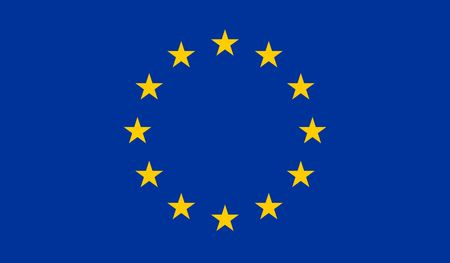
\includegraphics[height=5pt]{../_logos/eu-flag.jpg}
        \end{center}
    }
}

\begin{document}

\maketitle

\section{\eko{} \iRef{arXiv: 2202.02338}}

\begin{frame}{EKO}
    ciao
\end{frame}

\section{Intrinsic Charm in the Proton \iRef{submitted}}

\begin{frame}{EKO}
    ciao
\end{frame}

\section{\yadism{} \iRef{in preparation}}

\begin{frame}{EKO}
    ciao
\end{frame}

\begin{frame}{DIS coefficients}
    \vspace*{25pt}

    \begin{columns}
        \begin{column}{0.5\textwidth}
            \begin{table}[h!]
                \large
                \centering
                \begin{tabular}{c | c c c } 
                    NLO & light & heavy & intrinsic\\
                    \hline
                    NC & \cellcolor{green!25}\checkmark 
                       & \cellcolor{green!25}\checkmark 
                       & \cellcolor{green!25}\checkmark\\
                    CC & \cellcolor{green!25}\checkmark
                       & \cellcolor{green!25}\checkmark
                       & \cellcolor{blue!25}\checkmark\\
                    NNLO & & &\\
                    \hline
                    NC & \cellcolor{green!25}\checkmark
                       & \cellcolor{blue!25}partially tabulated
                       & \cellcolor{red!25}\ding{55}\\
                    CC & \cellcolor{green!25}\checkmark
                       & \cellcolor{yellow!25}tabulated
                       & \cellcolor{red!25}\ding{55}\\
                    N3LO & & &\\
                    \hline
                    NC & \cellcolor{yellow!25}\checkmark
                       &  & \\
                    CC & \cellcolor{yellow!25}\checkmark
                       &  & \\
                \end{tabular}
            \end{table}
            + FONLL (cf. \textit{matching conditions})
        \end{column}
        \begin{column}{0.5\textwidth}
            There is even another couple of levels of nesting:
            
            \setlist[description]{font=\quad\normalfont\bfseries\scshape\space}
            \begin{description}
                \item[Projections] $F_2$, $F_L$, and $F_3$
                \item[Channels] non-singlet, singlet, gluon
            \end{description}

            \vspace*{10pt}
            {
                \footnotesize
                But up to NNLO everything is equally available (while at N3LO
                it is not always true).
            }
        \end{column}
    \end{columns}

    \vspace*{10pt}

    So NC is currently implemented up to NNLO
    \iRef{\href{https://doi.org/10.1016/j.nuclphysb.2005.06.020}{VVM05}
    \href{https://doi.org/10.1016/j.physletb.2004.11.063}{MVV05}
    \href{https://doi.org/10.1016/S0550-3213(00)00045-6}{MV00}}
    light and NLO heavy \iRef{\href{https://arxiv.org/abs/1910.01536}{Hek19}}
    (i.e. both $O(a_s^2)$).
    Same for CC light
    \iRef{\href{https://doi.org/10.1016/j.nuclphysb.2007.09.022}{MRV08}
    \href{https://doi.org/10.1016/j.nuclphysb.2009.01.001}{MVV09}} and heavy
    (for which implementation is currently in progress).

    For both processes \textit{intrinsic} contributions are accounted at NLO.
    
    \vspace*{15pt}
    {
        \footnotesize
        \begin{flushright}
            \begin{tabular}{c c c c c} 
                \cellcolor{green!25}available & \cellcolor{blue!25}updated
                                            &\cellcolor{yellow!25}not yet implemented
                                            &\cellcolor{red!25}missing
                                            & not planned\\
                \hline
            \end{tabular}
        \end{flushright}
    }
\end{frame}

\section{Theory Prediction Pipeline}

\begin{frame}{EKO}
    ciao
\end{frame}

\begin{frame}[standout]
    Thank you for listening!
\end{frame}

\appendix

\begin{frame}{Anomalous Dimensions}
    Most of them were already available and used in APFEL, and they have been implemented in EKO:
    \begin{table}[h!]
        \centering
        \begin{tabular}{c c c c} 
            LO & NLO & NNLO & N3LO\\
            \hline
            \cellcolor{green!25}\checkmark & \cellcolor{green!25}\checkmark & \cellcolor{green!25}\checkmark & \cellcolor{red!25}\ding{55}\\
        \end{tabular}
    \end{table}
    
    We are just missing the N3LO expressions, required only for N3LO evolution
    (\textit{expected} to receive an approximation by \textbf{J. Vermaseren}
    and \textbf{A. Vogt}).

    \vspace*{15pt}
    There is \textit{no need for any extra modification} of EKO at N3LO, we
    just deserve to plug in the expressions.
\end{frame}

\begin{frame}{Scale Variations}
    Scale variations are implemented in \texttt{yadism} (\textbf{scheme C}) as completely
    factorized w.r.t. coefficients functions (instead of inlined).

    The actual ingredients needed to combine them are:
    \begin{itemize}
        \item splitting functions ($x$-space), one order less (NLO DIS requires LO $P$)
        \item beta function coefficients, two order less (NNLO DIS requires $\beta_0$)
        \item combination rules
    \end{itemize}

    \begin{table}[h!]
        \centering
        \begin{tabular}{c c c c c} 
             & NLO & NNLO & N3LO\\
            \hline
            $P^{(n-1)}$ &  \cellcolor{green!25}\checkmark & \cellcolor{green!25}\checkmark & \cellcolor{yellow!25}\checkmark\\
            $\beta^{n-2}$ &  & \cellcolor{green!25}\checkmark & \cellcolor{green!25}\checkmark\\
            rules & \cellcolor{green!25}\checkmark & \cellcolor{green!25}\checkmark & \cellcolor{yellow!25}\checkmark\\
            \hline
            \texttt{yadism} & \cellcolor{green!25}\checkmark & \cellcolor{green!25}\checkmark & \cellcolor{yellow!25}
        \end{tabular}
    \end{table}

    \vspace*{10pt}
    Actually there is one further step: to save time and precision \textbf{convolution}
    of splitting functions are \textbf{inlined}.

    This means they have to be computed analytically, and this requires some
    manual work.

    \metroset{block=fill}

    \begin{block}{\texttt{eko}}
        \textbf{scheme A} \checkmark is implemented, while \textbf{scheme B} \ding{55} is work-in-progress.
    \end{block}
\end{frame}

\begin{frame}{Matching Conditions}
definition\footnote{simplified version, full truth in \alert{\href{https://eko.readthedocs.io/en/latest/theory/Matching.html}{eko docs}}}:
    \begin{columns}
        \begin{column}{0.1\textwidth}\end{column}
        \begin{column}{0.4\textwidth}
            \begin{align*}
                \begin{pmatrix}
                    g \\ \Sigma \\ h^+            
                \end{pmatrix}
                &= 
                \begin{pmatrix}
                    gg & gq & gh \\
                    qg & ns_+ + ps & qh \\
                    hg & hq & hh
                \end{pmatrix}
                \begin{pmatrix}
                    g \\ \Sigma \\ h^+            
                \end{pmatrix}
                \\
                T_n &= ns_+ T_n \qquad\qquad  
            \end{align*}
        \end{column}
        \begin{column}{0.4\textwidth}
            \begin{align*}
                \begin{pmatrix}
                    V \\ h^-
                \end{pmatrix}
                &= 
                \begin{pmatrix}
                    ns_v & qh \\
                    hq & hh 
                \end{pmatrix}
                \begin{pmatrix}
                    V \\ h^-
                \end{pmatrix}
                \\
                V_n &= ns_- V_n
            \end{align*}
        \end{column}
        \begin{column}{0.1\textwidth}\end{column}
    \end{columns}

    status:
    \begin{table}[h!]
        \centering
        \begin{tabular}{c c c c c c c c c c c c c} 
             & nsv & ns- & ns+ & ps & qg & gq & gg & hq & hg & qh & gh & hh \\
            \hline
            NLO & \multicolumn{1}{|c}{} &  & \multicolumn{1}{c|}{} & & & & \cellcolor{blue!25}$\mu$ & & \cellcolor{blue!25}$\mu$ & & \cellcolor{blue!25}\checkmark+$\mu$\footnotemark[2] & \cellcolor{blue!25}\checkmark+$\mu$\footnotemark[2] \\
            \cline{2-4}
            NNLO & \multicolumn{3}{|c|}{\cellcolor{green!65!blue!25}\checkmark+$\mu$} & & \cellcolor{green!65!blue!25}\checkmark+$\mu$ & \cellcolor{green!65!blue!25}\checkmark+$\mu$ & \cellcolor{green!65!blue!25}\checkmark+$\mu$ & \cellcolor{green!65!blue!25}\checkmark+$\mu$\footnotemark[1] & \cellcolor{green!65!blue!25}\checkmark+$\mu$ & \cellcolor{red!25}\ding{55}\footnotemark[3] & \cellcolor{red!25}\ding{55}\footnotemark[3] & \cellcolor{red!25}\ding{55}\footnotemark[3] \\
            \cline{2-4}
            N3LO & \multicolumn{3}{|c|}{\cellcolor{yellow!25}\checkmark+$\mu$} & \cellcolor{yellow!25}\checkmark+$\mu$ & \cellcolor{yellow!25}\checkmark+$\mu$ & \cellcolor{yellow!25}\checkmark+$\mu$ & \cellcolor{yellow!65!red!25}$\sim$ & \cellcolor{yellow!25}\checkmark+$\mu$ & \cellcolor{yellow!65!red!25}$\sim$\\
            \cline{2-4} \\
        \end{tabular}
    \end{table}

    $\mu$ stands for the extra contribution given from taking a threshold
    different from quark mass, and it is proportional to $\log(\mu^2/m^2)$.

    \begin{enumerate}
        \item actually $\text{hq}_\text{ps}$
        \item taken from \textbf{NNPDF}, computed from \textbf{Kretzer \& Schienbein}
        \item \textbf{Kirill} about to compute
    \end{enumerate}
\end{frame}

\end{document}
